\chapter{Specyfikacja wewnętrzna}
\label{ch:05}

\section{Architektura systemu oraz przedstawienie idei}
Do realizacji projektu wykorzystano język C++ oraz bibliotekę OpenGL. Do~kompilacji programu wykorzystano system budowy CMake. Kod odpowiadający za~renderowanie obrazu napisany został w języku GLSL i wykonywany jest na karcie graficznej.
W pierwszej kolejności następuje utworzenie okna programu z~wykorzystaniem biblioteki GLFW. Kolejny krok to inicjalizacja biblioteki OpenGL przy~wykorzystaniu biblioteki GLAD i rozpoczęcie głównej pętli programu, w której obsługiwane są następujące czynności:
\begin{itemize}
\item obsługa klawiatury i myszki,
\item wyświetlenie i obsługa interfejsu użytkownika,
\item pobranie ustawień z interfejsu użytkownika i przekazanie ich do karty graficznej,
\item rozpoczęcie renderowania obrazu,
\item wyświetlenie uzyskanego obrazu.
\end{itemize}

Informacje o konfiguracji przekazywane są do jednostek cieniujących przy~wykorzystaniu zmiennych typu \ang{uniform}. Jednostka cieniująca wierzchołków tworzy prostokąt pokrywający cały ekran, na którym odbywa się renderowanie obrazu. Całość renderowania odbywa się w jednostce cieniującej fragmentów. Pierwszym etapem jest~obliczenie początkowej pozycji wiązki światła oraz jej kierunek dla każdego piksela. Uzyskane w ten sposób informacje o wiązce światła przekazywane są do funkcji \ang{render}. Funkcja ta odpowiada za następujące czynności:
\begin{itemize}
\item wywołanie funkcji algorytmu raymarching,
\item uzyskanie wektorów normalnych,
\item obliczenie koloru w zależności od rodzaju przeciętej wiązką światła powierzchni,
\item obliczenia związane z cieniem i cieniowaniem,
\item obliczenie końcowego koloru danego piksela,
\item zastosowanie korekcji gamma.
\end{itemize}

\section{Przegląd ważniejszych klas oraz struktur danych}
W programie jedną najważniejszych jest klasa \ang{Application}, która odpowiada za~inicjalizację całego programu oraz wykorzystanych bibliotek. Klasa ta zawiera główną pętlę programu, dodatkowo odpowiada za obsługę klawiatury i myszki. Deklaracja tej klasy została przedstawiona na rysunku \ref{fig:c++:application}.

\begin{figure}[H]
\centering
\begin{lstlisting}[language=C++]
class Application
{
public:
  Application();
  ~Application();

  void run();
  void processInput();

private:
  Window win;
  UI ui;
  Config config;
  Renderer renderer;
};
\end{lstlisting}
\caption{Deklaracja klasy \ang{Application}.}
\label{fig:c++:application}
\end{figure}

Równie ważną jest klasa \ang{Renderer}, która odpowiada za inicjalizację podstawowych elementów niezbędnych do rozpoczęcia renderowania, kompilację jednostek cieniujących oraz ich połączenie. Ponadto umożliwia przekazywanie konfiguracji do jednostek cieniujących i rozpoczęcie renderowania. Rysunek \ref{fig:c++:renderer} przedstawia deklarację tej klasy.

\begin{figure}[H]
\centering
\begin{lstlisting}[language=C++]
class Renderer
{
public:
  Renderer();
  ~Renderer();

  void update();
  void draw(const Config &c);

private:
  void updateUniforms(const Config &c);

  std::unique_ptr<GL::Program> program;
  std::unique_ptr<GL::Shader> vertexShader;
  GL::VAO vao;
};

\end{lstlisting}
\caption{Deklaracja klasy \ang{Renderer}.}
\label{fig:c++:renderer}
\end{figure}

Należy przytoczyć jeszcze klasę \ang{Window}, odpowiadającą za inicjalizację oraz obsługę okna aplikacji.
Deklaracja tej klasy widoczna jest na rysunku \ref{fig:c++:window}.

\begin{figure}[H]
\centering
\begin{lstlisting}[language=C++]
class Window
{
public:
  Window();
  Window(unsigned width, unsigned height);
  ~Window();

  bool shouldClose() const;
  void pollEvents();
  void swapBuffers();

  operator GLFWwindow *() const { return w; }

private:
  GLFWwindow *w;
};
\end{lstlisting}
\caption{Deklaracja klasy \ang{Renderer}.}
\label{fig:c++:window}
\end{figure}

\section{Przegląd ważniejszych algorytmów}

Algorytm \ang{raymarching} jest najważniejszym z algorytmów wykorzystanych w~programie. Jego rola polega na stopniowym
przesuwaniu wiązki światła do momentu przecięcia z dowolnym punktem powierzchni sceny. Sam algorytm wykorzystuje podane parametry, którymi są początkowa pozycja wiązki światła oraz jej kierunek. Jego~końcowy wynik to odległość, którą musi przebyć wiązka by preciąć najbliższą powierzchnię. Algorytm ten wykorzystuje pomocniczą funkcję
\ang{map()}, która zwraca odległość między podanym punktem a najbliższą powierzchnią sceny. Kod tej funkcji zmienia się w zależności od renderowanej sceny, dlatego pominięto jej pseudokod.
Rysunek \ref{fig:pseudokod:raymarching} przedstawia pseudokod tego algorytmu.

\begin{figure}[H]
\centering
\begin{lstlisting}[language=C]
float raymarch(vec3 rayOrigin, vec3 rayDirection)
{
  float distance = 0.0;

  for (int i = 0; i < MAX_STEPS; i++) {
    vec3 pos = rayOrigin + rayDirection * distance;
    float d = map(pos);
    distance += d;

    if (abs(d) < EPSILON) {
      return distance;
    }
    if (distance > MAX_DIST) {
      break;
    }
  }
  return MAX_DIST;
}
\end{lstlisting}
\caption{Pseudokod algorytmu renderowania metodą \ang{raymarching}.}
\label{fig:pseudokod:raymarching}
\end{figure}

Aby uzyskać efekt cienia, wykorzystano modyfikację tego algorytmu, w punkcie przecięcia wiązki zostaje wysłana nowa wiązka skierowana w kierunku źródła światła. Na~podstawie informacji o przecięciu ze sceną tej wiązki można określić czy dany punkt jest~oświetlony. Dodatkowo wykorzystując wzór \ref{eq:r-shadow} można uzyskać efekt ,,miękkich'' cieni przy niewielkim koszcie obliczeń \cite{bib:iqsoftshadow}.
Rysunek \ref{fig:pseudokod:shadow} przedstawia pseudokod z~wykorzystaniem ,,miękkich'' cieni.
\begin{equation}
\label{eq:r-shadow}
r = min(\frac{map(p)}{\text{distance}})
\end{equation}
\begin{figure}[H]
\centering
\begin{lstlisting}[language=C]
float shadow(vec3 rayOrigin)
{
  float distance = 0.0;
  float minR = MAX_DIST;

  for (int i = 0; i < MAX_STEPS; i++) {
    vec3 pos = ro + sunDir * distance;
    float d = map(pos);

    float r = d/depth;
    minR = min(r, minR);

    depth += d;

    if (abs(d) < EPSILON)
      return 0.0;

    if (d > MAX_DIST) break;
  }
  return smoothstep(0.0, 1.0, minR);
}
\end{lstlisting}
\caption{Pseudokod modyfikacji algorytmu \ang{raymarching} wykorzystany do obliczenia cieni.}
\label{fig:pseudokod:shadow}
\end{figure}

Różnice wynikające z zastosowania wzoru \ref{eq:r-shadow} przedstawia rysunek \ref{fig:shadow-comp}

\begin{figure}[H]
\centering
\subfloat[zwykłe cienie]{
  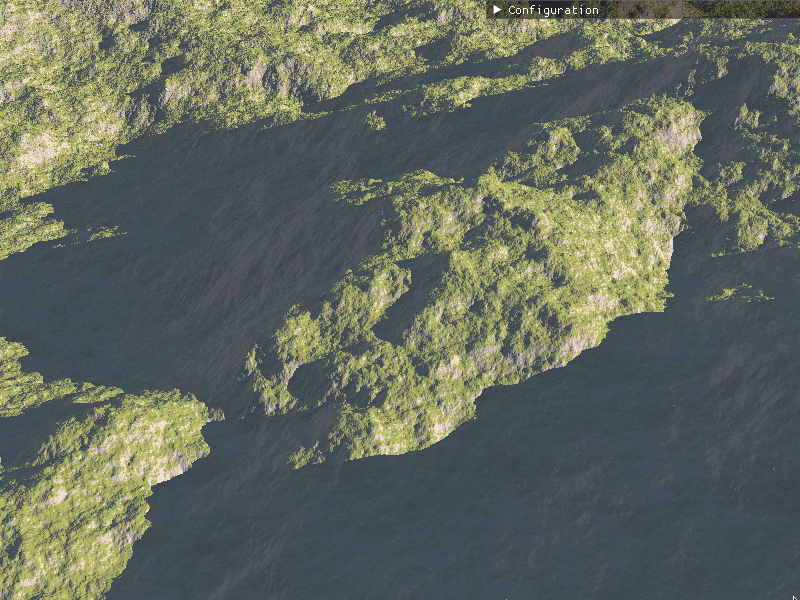
\includegraphics[width=0.5\textwidth]{./graf/shadow.png}
}
\subfloat[,,miękkie'' cienie]{
  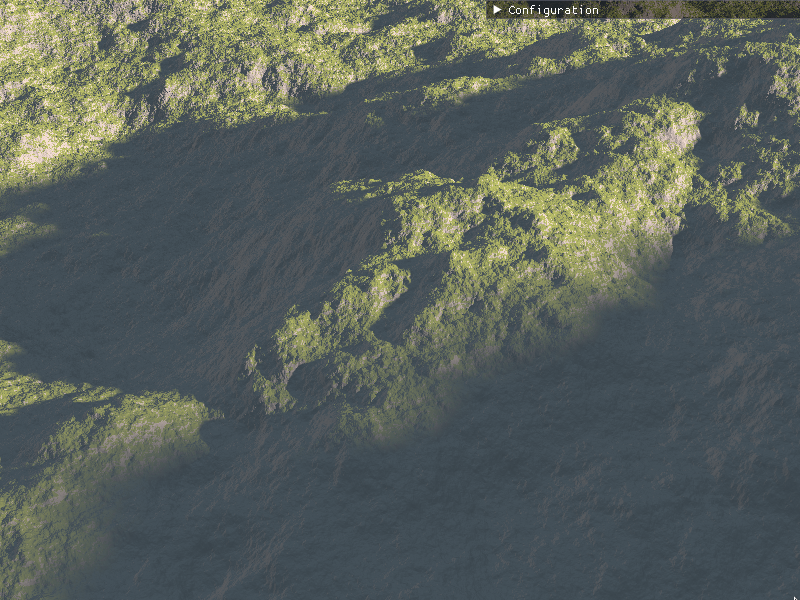
\includegraphics[width=0.5\textwidth]{./graf/shadowsmooth.png}
}
%% 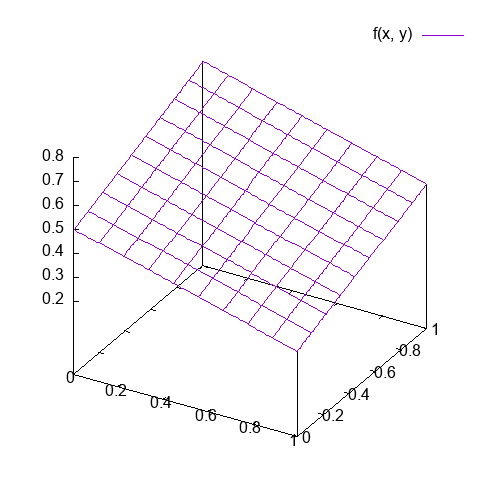
\includegraphics[width=0.65\textwidth]{./graf/plot/bilinear.png}
\caption{Porównanie wyników metod renderowania cieni}
\label{fig:shadow-comp}
\end{figure}

Kolejną wykorzystaną modyfikacją algorytmu raymarching jest funkcja odpowiadająca za renderowanie chmur, której pseudokod jest widoczny na rysunku \ref{fig:pseudokod:cloud}. Działanie takie, sprawia, że algorytm przecinając powierzchnię nie przerywa pracy, a zaczyna obliczać jej średnią gęstość. Efektem takiego rozwiązania jest uzysanie bardziej naturalnego wyglądu chmur, jak to przedstwiono na rysunku \ref{fig:clouds}.

\begin{figure}[H]
\centering
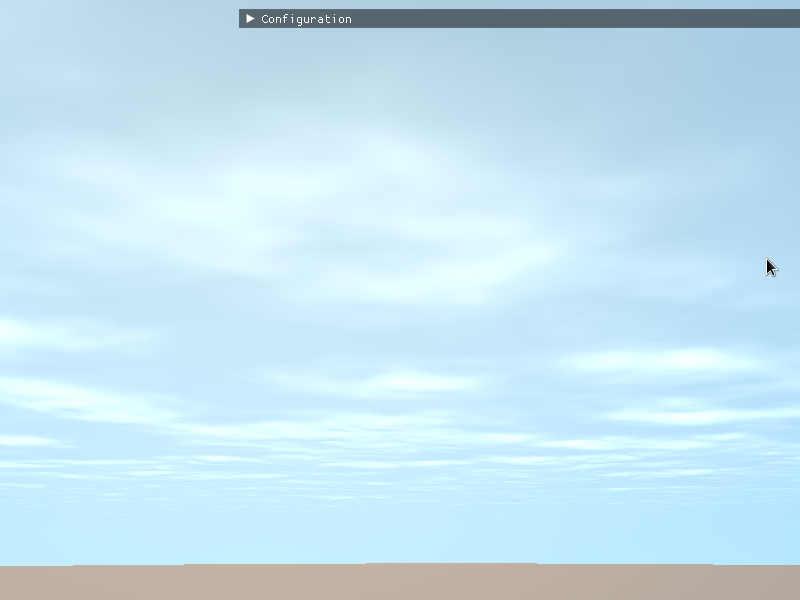
\includegraphics[width=1\textwidth]{./graf/clouds.png}
\caption{Renderowanie chmur.}
\label{fig:clouds}
\end{figure}

\begin{figure}[H]
\centering
\begin{lstlisting}[language=C]
vec4 raymarchClouds(vec3 ro, vec3 rd)
{
  float depth = 0.0; // total traveled distance
  float prec = EPSILON; // precision
  float density = 0.0;
  int densitySamples = 0;
  float absorption = 100.0;
  vec3 color = vec3(0.0);
  float hit = 0.0;

  for (int i = 0; i < cloudsMaxSteps; i++) {
    vec3 pos = ro + rd * depth;
    if (rd.y > 0 && pos.y > (cloudAltitude + cloudHeight)) break;
    if (rd.y < 0 && pos.y < (cloudAltitude - cloudHeight)) break;

    float d = cloudMap(pos);
    if (d < 0) {
      hit = 1.0;
      density += cloudDensityScaling * abs(d);
      densitySamples += 1;
      depth += STEP_SIZE;
    } else {
      depth += abs(d);
    }
  }
  if (densitySamples > 0)
    color = vec3(1.0) * smoothstep(0.0, 1.0, density/densitySamples);
  return vec4(hit, color);
}
\end{lstlisting}
\caption{Pseudokod modyfikacji algorytmu \ang{raymarching} wykorzystany do~renderowania chmur.}
\label{fig:pseudokod:cloud}
\end{figure}







%% \subchapter{Szczególy implementacji wybranych fragmentów kodu}
%% \begin{i%% temize}
%% \item przedstawienie idei
%% \item architektura systemu
%% \item komponenty, moduły, biblioteki, przegląd ważniejszych klas (jeśli występują)
%% \item opis struktur danych (i organizacji baz danych)
%% \item przegląd ważniejszych algorytmów (jeśli występują)
%% \item szczegóły implementacji wybranych fragmentów, zastosowane wzorce projektowe
%% \item diagramy UML
%% \end{itemize}

% % % % % % % % % % % % % % % % % % % % % % % % % % % % % % % % % % %
% Pakiet minted wymaga odkomentowania w pliku config/settings.tex   %
% importu pakietu minted: \usepackage{minted}                       %
% i specjalnego kompilowania:                                       %
% pdflatex -shell-escape praca                                      %
% % % % % % % % % % % % % % % % % % % % % % % % % % % % % % % % % % %


%% Krótka wstawka kodu w linii tekstu jest możliwa, np.  \lstinline|int a;| (biblioteka \texttt{listings})% lub  \mintinline{C++}|int a;| (biblioteka \texttt{minted})
%% .
%% Dłuższe fragmenty lepiej jest umieszczać jako rysunek, np. kod na rys \ref{fig:pseudokod:listings}% i rys. \ref{fig:pseudokod:minted}
%% , a naprawdę długie fragmenty – w załączniku.


%% \begin{figure}
%% \centering
%% \begin{lstlisting}
%% class test : public basic
%% {
%%     public:
%%       test (int a);
%%       friend std::ostream operator<<(std::ostream & s,
%%                                      const test & t);
%%     protected:
%%       int _a;

%% };
%% \end{lstlisting}
%% \caption{Pseudokod w \texttt{listings}.}
%% \label{fig:pseudokod:listings}
%% \end{figure}

%% %\begin{figure}
%% %\centering
%% %\begin{minted}[linenos,frame=lines]{c++}
%% %class test : public basic
%% %{
%% %    public:
%% %      test (int a);
%% %      friend std::ostream operator<<(std::ostream & s,
%% %                                     const test & t);
%% %    protected:
%% %      int _a;
%% %
%% %};
%% %\end{minted}
%% %\caption{Pseudokod w \texttt{minted}.}
%% %\label{fig:pseudokod:minted}
%% %\end{figure}
